
\section*{CHƯƠNG 3. THIẾT KẾ HỆ THỐNG}
\setcounter{section}{3}
\setcounter{subsection}{0} %LƯU Ý MỖI LẦN THÊM CHƯƠNG MỚI CẦN THÊM CÂU NÀY ĐỂ RESET THỨ TỰ CỦA SUBSECTON VỀ 1
\setcounter{table}{0} % LƯU Ý SAU MỖI LẦN GỌI BẢNG HAY HÌNH ẢNH PHẢI THÊM CÂU NÀY ĐỂ RESET THỨ TỰ
\setcounter{figure}{0} %% LƯU Ý SAU MỖI LẦN GỌI BẢNG HAY HÌNH ẢNH PHẢI THÊM CÂU NÀY ĐỂ RESET THỨ TỰ
\addcontentsline{toc}{section}{\numberline{}CHƯƠNG 3. THIẾT KẾ HỆ THỐNG}

Ở chương này, chúng em mô tả quá trình thiết kế hệ thống từ tổng quan đến chi tiết, dựa trên phân tích ở Chương 2.
Mở đầu là xây dựng sơ đồ kiến trúc hệ thống.
Tiếp theo, chương tập trung vào thiết kế giao diện người dùng và các chức năng chính cho website cùng server.
Nội dung chính được thể hiện qua hình ảnh và sơ đồ minh họa, không chỉ mô tả chi tiết luồng hoạt động mà còn làm rõ cách các thành phần trong hệ thống phối hợp, hỗ trợ lẫn nhau.
\subsection{Sơ đồ tổng quan kiến trúc của hệ thống}

\begin{figure}[H]
	\centering
	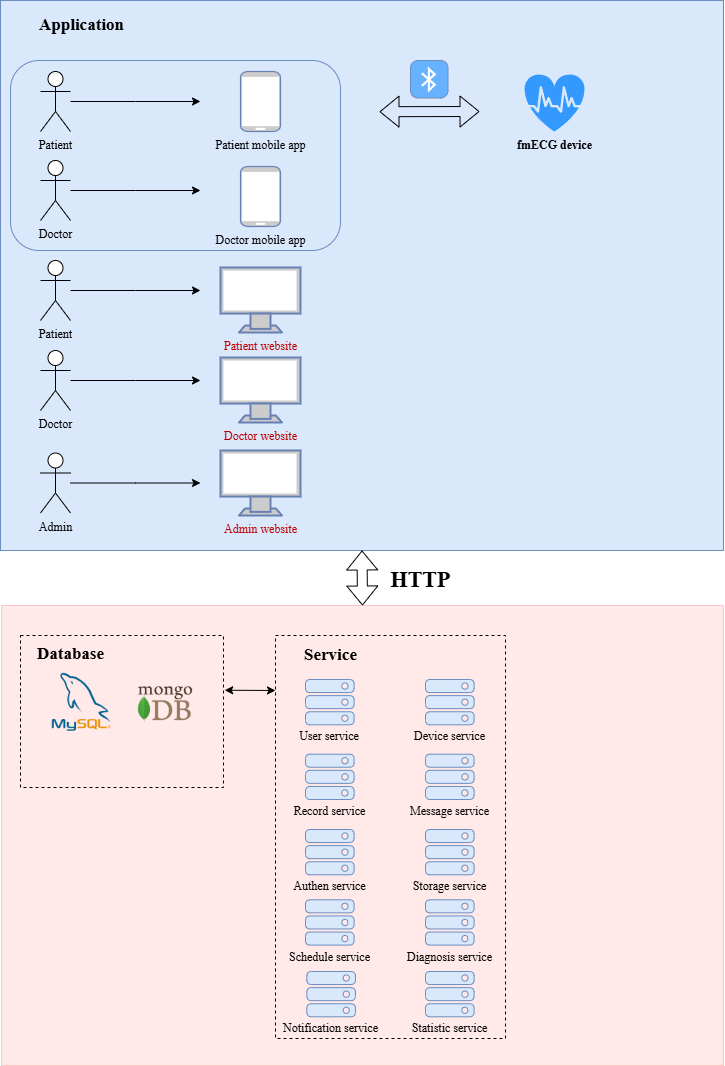
\includegraphics[width=12cm,height=16cm]{Images/System/fmECG_architecture-System_Architecture.drawio.png}
	\caption[Tổng quan kiến trúc hệ thống]{\bfseries \fontsize{12pt}{0pt}\selectfont Tổng quan kiến trúc hệ thống}
	\label{fmECG_architecture-System} %đặt tên cho ảnh
\end{figure}
Hệ thống được chia thành ba phần chính: Thiết bị (Device), Máy chủ (Server) và Ứng dụng (bao gồm web và app).
Mỗi thành phần đảm nhiệm một vai trò quan trọng, cùng phối hợp để đảm bảo hoạt động của toàn bộ hệ thống như được minh họa trong hình vẽ.

Hình \ref{fmECG_architecture-System} thể hiện ba phần:

\begin{adjustwidth}{1.5em}{}
	\begin{itemize}
		\item Device (Thiết bị): Gồm các thiết bị phần cứng đo điện tim, có khả năng kết nối với ứng dụng di động của bệnh nhân thông qua Bluetooth.
		\item Application (Ứng dụng): Bao gồm ứng dụng di động và website, phục vụ nhu cầu sử dụng của bệnh nhân, bác sĩ và quản trị viên.
		\item Server (Máy chủ): Chứa các dịch vụ (Services) xử lý yêu cầu từ ứng dụng và quản lý cơ sở dữ liệu.
	\end{itemize}
\end{adjustwidth}

Trong sơ đồ kiến trúc hệ thống, bệnh nhân sử dụng ứng dụng di động (Mobile App) để kết nối trực tiếp với thiết bị (Device).
Ứng dụng di động thuộc Khối Ứng dụng (Application), chịu trách nhiệm giao tiếp với Khối Máy chủ (Server) thông qua các API và giao thức HTTP.
Khi nhận được yêu cầu từ Application, Server sẽ thực hiện xử lý dữ liệu thông qua các dịch vụ (Services) được thiết kế riêng biệt.
Tùy theo loại yêu cầu, các dịch vụ này sẽ truy xuất hoặc cập nhật dữ liệu trong cơ sở dữ liệu, sau đó gửi kết quả phản hồi cho người dùng,
hoàn thiện quá trình tương tác giữa người dùng và hệ thống.\begin{adjustwidth}{1.5em}{}
	\begin{itemize}
		\item Authen Service: Đảm nhận các nhiệm vụ liên quan đến bảo mật hệ thống, bao gồm mã hóa dữ liệu nhạy cảm, tạo và xác thực token để đảm bảo tính an toàn khi truy cập,
		      quản lý phân quyền người dùng đối với API,và thực hiện mã hóa thông tin trước khi lưu trữ nhằm ngăn chặn rò rỉ dữ liệu.
		\item User Service: Xử lý toàn bộ các thao tác liên quan đến người dùng, như tạo tài khoản mới, xác thực thông tin đăng nhập, lấy thông tin cá nhân của người dùng,
		      đồng thời hỗ trợ cập nhật và chỉnh sửa thông tin cá nhân khi cần thiết.
		\item Device Service: Chịu trách nhiệm quản lý thiết bị, bao gồm các chức năng như thêm mới, chỉnh sửa thông tin, xóa thiết bị,
		      và cập nhật tình trạng thiết bị hoặc thông số liên quan để đảm bảo thiết bị hoạt động đúng trong hệ thống.
		\item Storage Service: Quản lý và vận hành hệ thống lưu trữ dữ liệu, bao gồm lưu trữ file, tài liệu, và các thông tin quan trọng của hệ thống.
		      Đồng thời, đảm bảo tính nhất quán của dữ liệu thông qua cơ chế xử lý race condition, khóa truy cập và đồng bộ hóa dữ liệu trong các trường hợp truy cập đồng thời,
		      cũng như tối ưu hóa hiệu suất lưu trữ và truy xuất dữ liệu.
		\item Record Service: Xử lý các dữ liệu liên quan đến phiên đo, bao gồm thêm mới, cập nhật, xóa dữ liệu, và xử lý các file đo được từ thiết bị trước khi lưu trữ hoặc gửi đến người dùng.
		\item Message Service: Quản lý toàn bộ các yêu cầu liên quan đến nhắn tin, bao gồm gửi, nhận, lưu trữ tin nhắn, hỗ trợ các nhóm trò chuyện giữa những người dùng trong hệ thống.
		\item Schedule Service: Đảm nhiệm việc quản lý lịch khám, bao gồm đặt lịch và xử lý các phản hồi liên quan, nhằm đảm bảo quy trình đặt lịch diễn ra mượt mà giữa bệnh nhân, bác sĩ và hệ thống.
		\item Diagnosis Service: Quản lý các tác vụ liên quan đến chẩn đoán, bao gồm thêm mới và chỉnh sửa thông tin chẩn đoán cho bệnh nhân, đảm bảo dữ liệu chính xác và hỗ trợ quá trình điều trị hiệu quả.
		\item Notification Service: Đảm bảo quản lý hiệu quả các thông báo cho người dùng, từ việc gửi thông báo sự kiện, cảnh báo, đến nhắc nhở,
		      giúp người dùng cập nhật kịp thời các thông tin quan trọng từ hệ thống.
		\item Statistic Service: Chịu trách nhiệm tổng hợp số liệu thống kê trong hệ thống, bao gồm số lượng người dùng (bệnh nhân và bác sĩ),
		      số thiết bị, và dữ liệu phiên đo theo từng tháng, nhằm cung cấp thông tin phục vụ quản lý hiệu quả.
	\end{itemize}
\end{adjustwidth}

Dưới đây là mô tả chi tiết về các phần nhỏ hơn trong kiến trúc hệ thống, được xây dựng dựa trên các đối tượng chính đã phân tích.
\newpage
\subsection{Sơ đồ khối phần mềm}

\subsubsection{Website dành cho bệnh nhân}
\begin{figure}[H]
	\centering
	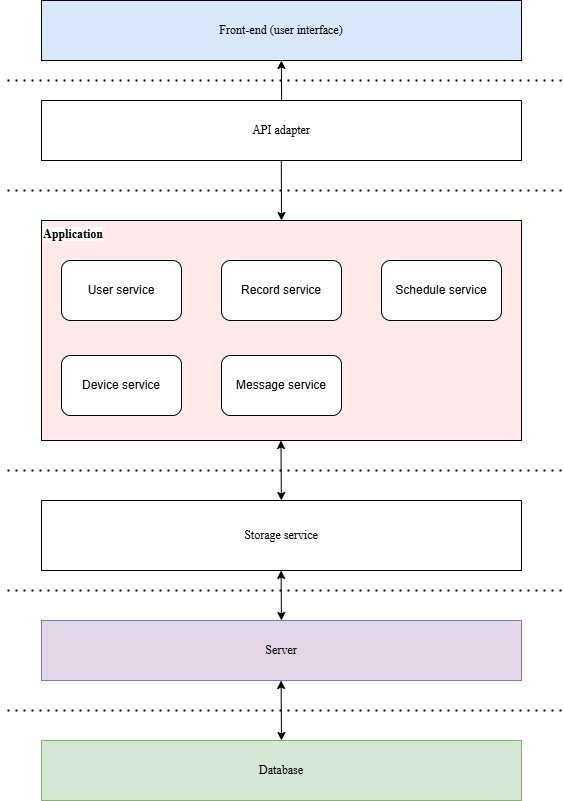
\includegraphics[width=12cm,height=15cm]{Images/System/fmECG_architecture-Patient.drawio.png}
	\caption[Sơ đồ khối Website dành cho bệnh nhân]{\bfseries \fontsize{12pt}{0pt}\selectfont Sơ đồ khối Website dành cho bệnh nhân}
	\label{fmECG_architecture-Patient} %đặt tên cho ảnh
\end{figure}
Tầng trên cùng trong sơ đồ hình \ref{fmECG_architecture-Patient} là User Interface (Giao diện người dùng), nơi bệnh nhân trực tiếp tương tác với hệ thống thông qua API Adapter để gửi yêu cầu và nhận phản hồi.
Các yêu cầu này được xử lý bởi các Services chính, bao gồm User Service, Device Service, Record Service, Schedule Service, Diagnosis Service, Notification Service và Storage Service.

Những Services này được thiết kế nhằm đáp ứng các nhu cầu của bệnh nhân, từ quản lý thông tin cá nhân, mượn và trả thiết bị, theo dõi lịch sử dữ liệu phiên đo, cho đến việc quản lý lịch khám,
tra cứu thông tin chẩn đoán cho từng lịch khám. Ngoài ra, hệ thống còn đảm bảo việc gửi thông báo nhắc nhở kịp thời và hỗ trợ bệnh nhân trao đổi thông tin với bác sĩ một cách liền mạch và hiệu quả.

\subsubsection{Website dành cho bác sĩ}
\begin{figure}[H]
	\centering
	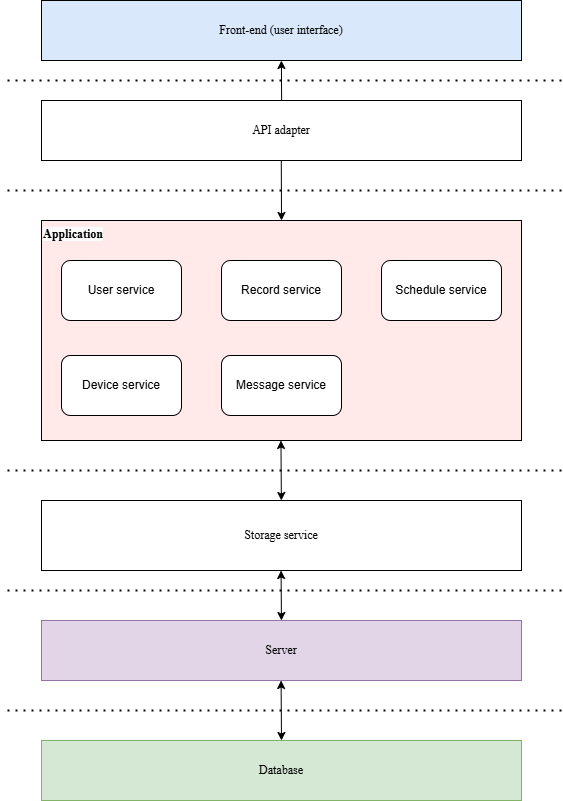
\includegraphics[width=12cm,height=15cm]{Images/System/fmECG_architecture-Doctors.drawio.png}
	\caption[Sơ đồ khối Website dành cho bác sĩ]{\bfseries \fontsize{12pt}{0pt}\selectfont Sơ đồ khối Website dành cho bác sĩ}
	\label{fmECG_architecture-Doctor} %đặt tên cho ảnh
\end{figure}

Tương tự với bệnh nhân, sơ đồ hình \ref{fmECG_architecture-Doctor} được xây dựng để hỗ trợ bác sĩ thực hiện các nhiệm vụ chuyên môn thông qua giao diện người dùng và API Adapter, đảm bảo việc xử lý thông tin diễn ra nhanh chóng và hiệu quả.

Các Services chính, bao gồm User Service, Device Service, Record Service, Schedule Service, Diagnosis Service, Notification Service và Storage Service, đóng vai trò quan trọng trong việc hỗ trợ bác sĩ.
Các nhiệm vụ được tập trung vào việc theo dõi và phân tích dữ liệu phiên đo từ bệnh nhân, quản lý lịch khám, chấp nhận hoặc từ chối yêu cầu đặt lịch, ghi nhận thông tin chẩn đoán, và trao đổi trực tiếp với bệnh nhân.
Hơn nữa, hệ thống cung cấp khả năng tự động gửi thông báo về lịch khám và nhắc nhở các cuộc khám sắp tới, giúp bác sĩ quản lý thời gian và công việc hiệu quả hơn.

Cách tiếp cận này không chỉ hỗ trợ bác sĩ tổ chức công việc thuận lợi mà còn góp phần nâng cao hiệu quả điều trị cho bệnh nhân.

\subsubsection{Website cho quản trị viên}
\begin{figure}[H]
	\centering
	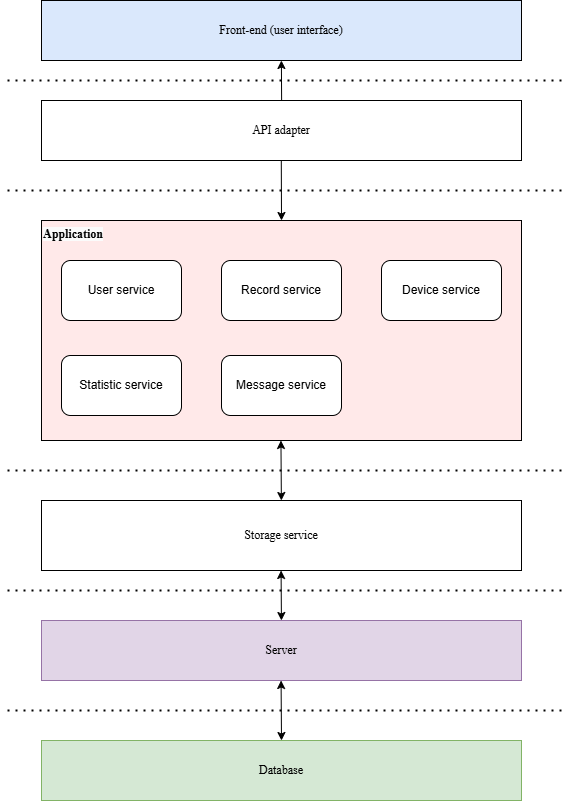
\includegraphics[width=12cm,height=15cm]{Images/System/fmECG_architecture-Admin.drawio.png}
	\caption[Sơ đồ khối Website dành cho quản trị viên]{\bfseries \fontsize{12pt}{0pt}\selectfont Sơ đồ khối Website dành cho quản trị viên}
	\label{fmECG_architecture-Admin} %đặt tên cho ảnh
\end{figure}
Về cơ bản, website dành cho admin được thiết kế với cấu trúc tương tự như website dành cho bác sĩ và bệnh nhân nhưng với quyền hạn mở rộng hơn.
Admin có thể quản lý toàn bộ thông tin người dùng, dữ liệu phiên đo, theo dõi các thống kê tổng quan của hệ thống, kiểm soát thông tin và kết quả chẩn đoán từ các lịch khám,
đồng thời điều hành việc mượn trả thiết bị một cách linh hoạt và hiệu quả.

\subsection{Thiết kế cơ sở dữ liệu}

\subsubsection{Chuyển đổi từ mô hình thực thể liên kết sang mô hình quan hệ}
Dựa trên bảng mô tả các thực thể và thuộc tính, chúng em tiến hành chuyển đổi từ mô hình thực thể liên kết thành mô hình quan hệ như sau.

\begin{itemize}
	\item Tài khoản đăng nhập (\textbf{ID tài khoản đăng nhập}, Địa chỉ email đăng ký, Mật khẩu truy cập)
	\item Token đăng nhập (\textbf{ID token đăng nhập}, ID tài khoản đăng nhập, Token làm mới, Hạn sử dụng, Trạng thái token)
	\item Vai trò người dùng (\textbf{ID vai trò}, Tên vai trò)
	\item Trạng thái hoạt động (\textbf{ID trạng thái người dùng}, Mô tả trạng thái người dùng)
	\item Người dùng (\textbf{ID người dùng}, ID tài khoản đăng nhập, ID vai trò người dùng, ID trạng thái hoạt động, Tên đầy đủ, Ngày tháng năm sinh, Giới tính, Số liên lạc, Đường dẫn ảnh đại diện, Thông tin bổ sung)
	\item Loại thiết bị (\textbf{ID loại thiết bị}, Tên loại thiết bị)
	\item Trạng thái thiết bị (\textbf{ID trạng thái thiết bị}, Mô tả trạng thái thiết bị)
	\item Thiết bị (\textbf{ID thiết bị}, ID người dùng thiết bị, ID loại thiết bị, ID trạng thái thiết bị, Tên thiết bị, Thông tin chi tiết về thiết bị, Ngày bắt đầu thời gian mượn, Ngày kết thúc thời gian mượn)
	\item Thông số kỹ thuật (\textbf{ID thông số kỹ thuật}, ID thiết bị, Loại thông số, Tên thông số, Giá trị thông số, Mô tả chi tiết thông số)
	\item Dữ liệu phiên đo (\textbf{ID dữ liệu phiên đo}, ID bệnh nhân, ID thiết bị, Loại bản ghi, Đường dẫn lưu trữ dữ liệu phiên đo, Thời gian bắt đầu thu thập dữ liệu, Thời gian kết thúc thu thập dữ liệu)
	\item Trạng thái lịch khám (\textbf{ID trạng thái lịch khám}, Mô tả trạng thái lịch khám)
	\item Kết quả lịch khám (\textbf{ID kết quả lịch khám}, Mô tả kết quả lịch khám)
	\item Lịch khám (\textbf{ID lịch khám}, ID bệnh nhân, ID bác sĩ, ID trạng thái lịch khám, ID kết quả lịch khám, Thời gian bắt đầu lịch khám, Thời gian kết thúc lịch khám)
	\item Thông báo liên quan đến lịch khám (\textbf{ID thông báo}, ID lịch khám, Loại thông báo, Nội dung thông báo, Trạng thái thông báo, Trạng thái đã xem, Lý do từ chối lịch khám)
	\item Chẩn đoán (\textbf{ID chẩn đoán}, ID lịch khám, Thông tin chẩn đoán)
	\item Tin nhắn (\textbf{ID tin nhắn}, ID người gửi, ID nhóm trò chuyện nhận tin nhắn, Nội dung tin nhắn, Thời gian gửi tin nhắn)
	\item Nhóm trò chuyện (\textbf{ID nhóm trò chuyện}, Tên nhóm trò chuyện, Người tạo nhóm, Danh sách thành viên nhóm, Sự kiện gửi tin nhắn, Sự kiện nhận tin nhắn)

\end{itemize}

\subsubsection{Chuẩn hoá 3NF}
Các bảng đã được thiết kế theo nguyên tắc chuẩn hoá 3NF, vì không có thuộc tính lặp lại và các thuộc tính không phụ thuộc vào một tập hợp con của khóa chính.

\paragraph{Chuẩn hoá bảng Người dùng}
\mbox{}
\begin{table}[H]
	\caption{\bfseries \fontsize{12pt}{0pt}\selectfont Bảng chuẩn hoá bảng Người dùng}
	\centering
	\begin{tabularx}{0.9\textwidth}{|X|X|}
		\hline
		\textbf{Danh sách thuộc tính}                & ID người dùng, ID tài khoản, Tên người dùng, Ngày sinh, Giới tính, Số điện thoại, Quyền, Trạng thái, Đường dẫn lưu trữ ảnh, Thông tin người dùng                                  \\
		\hline
		\textbf{Quy tắc nghiệp vụ}                   & \textbf{Phụ thuộc hàm}                                                                                                                                                            \\
		\hline
		Mỗi người dùng có một ID riêng, có duy nhất ID tài khoản, tên, ngày sinh, giới tính, số điện thoại, quyền,
		trạng thái, đường dẫn lưu trữ ảnh, thông tin & \parbox[t]{\linewidth}{$\text{ID người dùng} \rightarrow$ ID tài khoản, Tên người dùng, Ngày sinh, Giới Tính, Số điện thoại, Quyền, Trạng thái, Đường dẫn lưu trữ ảnh, Thông tin} \\
		\hline
		\multicolumn{2}{|X|}{$\Rightarrow \text{Khoá chính của bảng: ID người dùng}$}                                                                                                                                                    \\
		\multicolumn{2}{|X|}{$\Rightarrow \text{Bảng Người dùng đã ở 3NF}$}                                                                                                                                                              \\
		\hline
	\end{tabularx}
\end{table}

\paragraph{Chuẩn hoá bảng Tài khoản}
\mbox{}
\begin{table}[H]
	\caption{\bfseries \fontsize{12pt}{0pt}\selectfont Bảng chuẩn hoá bảng Tài khoản}
	\centering
	\begin{tabularx}{0.9\textwidth}{|X|X|}
		\hline
		\textbf{Danh sách thuộc tính} & ID tài khoản, Email, Mật khẩu                                             \\
		\hline
		\textbf{Quy tắc nghiệp vụ}    & \textbf{Phụ thuộc hàm}                                                    \\
		\hline
		Mỗi tài khoản có một ID riêng, có duy nhất email, mật khẩu
		                              & \parbox[t]{\linewidth}{$\text{ID tài khoản} \rightarrow$ Email, mật khẩu} \\
		\hline
		\multicolumn{2}{|X|}{$\Rightarrow \text{Khoá chính của bảng: ID tài khoản}$}                              \\
		\multicolumn{2}{|X|}{$\Rightarrow \text{Bảng Tài khoản đã ở 3NF}$}                                        \\
		\hline
	\end{tabularx}
\end{table}

% \paragraph{Chuẩn hoá bảng Token đăng nhập}
% \mbox{}
% \begin{table}[H]
%   \caption{\bfseries \fontsize{12pt}{0pt}\selectfont Bảng chuẩn hoá bảng Token đăng nhập}
%   \centering
%   \begin{tabularx}{0.9\textwidth}{|X|X|}
%     \hline
%     \textbf{Danh sách thuộc tính} & ID token, ID tài khoản, Token truy cập, Token làm mới \\
%     \hline
%     \textbf{Quy tắc nghiệp vụ} & \textbf{Phụ thuộc hàm} \\
%     \hline
%     Mỗi người dùng có một ID token riêng, có duy nhất ID tài khoản, token truy cập và token làm mới 
%     & \parbox[t]{\linewidth}{$\text{ID token} \rightarrow$ ID tài khoản, Token truy cập, Token làm mới} \\
%     \hline
%     \multicolumn{2}{|X|}{$\Rightarrow \text{Khoá chính của bảng: ID token đăng nhập}$} \\
%     \multicolumn{2}{|X|}{$\Rightarrow \text{Bảng Token  đã ở 3NF}$} \\
%     \hline
%   \end{tabularx}
% \end{table}

\paragraph{Chuẩn hoá bảng Thiết bị}
\mbox{}
\begin{table}[H]
	\caption{\bfseries \fontsize{12pt}{0pt}\selectfont Bảng chuẩn hoá bảng Thiết bị}
	\centering
	\begin{tabularx}{0.9\textwidth}{|X|X|}
		\hline
		\textbf{Danh sách thuộc tính} & ID thiết bị, ID người dùng thiết bị, Tên thiết bị,
		Loại thiết bị, Thông tin thiết bị, Trạng thái thiết bị, Ngày bắt đầu sử dụng, Ngày kết thúc sử dụng                           \\
		\hline
		\textbf{Quy tắc nghiệp vụ}    & \textbf{Phụ thuộc hàm}                                                                        \\
		\hline
		Mỗi thiết bị khi được sử dụng sẽ có một ID thiết bị riêng, có duy nhất tên thiết bị, loại thiết bị, thông tin thiết bị,
		ID người dùng thiết bị, trạng thái thiết bị, ngày bắt đầu sử dụng, ngày kết thúc sử dụng
		                              & \parbox[t]{\linewidth}{$\text{ID thiết bị} \rightarrow$ ID người dùng thiết bị, Tên thiết bị,
		Loại thiết bị, Thông tin thiết bị, Trạng thái thiết bị, Ngày bắt đầu sử dụng, Ngày kết thúc sử dụng}                          \\
		\hline
		\multicolumn{2}{|X|}{$\Rightarrow \text{Khoá chính của bảng: ID thiết bị}$}                                                   \\
		\multicolumn{2}{|X|}{$\Rightarrow \text{Bảng Thiết bị đã ở 3NF}$}                                                             \\
		\hline
	\end{tabularx}
\end{table}

\paragraph{Chuẩn hoá bảng Thông số thiết bị}
\mbox{}
\begin{table}[H]
	\caption{\bfseries \fontsize{12pt}{0pt}\selectfont Bảng chuẩn hoá bảng Thông số thiết bị}
	\centering
	\begin{tabularx}{0.9\textwidth}{|X|X|}
		\hline
		\textbf{Danh sách thuộc tính} & ID thông số, ID thiết bị, Tên thông số, Giá trị,
		Thông tin thông số, Loại thông số                                                                                           \\
		\hline
		\textbf{Quy tắc nghiệp vụ}    & \textbf{Phụ thuộc hàm}                                                                      \\
		\hline
		Mỗi thông số thiết bị sẽ có một ID thông số riêng, có duy nhất Tên thông số, ID thiết bị, Giá trị,
		Thông tin thông số, Loại thông số
		                              & \parbox[t]{\linewidth}{$\text{ID thông số} \rightarrow$ Tên thông số, ID thiết bị, Giá trị,
		Thông tin thông số, Loại thông số}                                                                                          \\
		\hline
		\multicolumn{2}{|X|}{$\Rightarrow \text{Khoá chính của bảng: ID thông số thiết bị}$}                                        \\
		\multicolumn{2}{|X|}{$\Rightarrow \text{Bảng Thiết bị đã ở 3NF}$}                                                           \\
		\hline
	\end{tabularx}
\end{table}

\paragraph{Chuẩn hoá bảng Bản ghi dữ liệu}
\mbox{}
\begin{table}[H]
	\caption{\bfseries \fontsize{12pt}{0pt}\selectfont Bảng chuẩn hoá bảng Bản ghi dữ liệu}
	\centering
	\begin{tabularx}{0.9\textwidth}{|X|X|}
		\hline
		\textbf{Danh sách thuộc tính} & ID bản ghi dữ liệu, ID người dùng, ID thiết bị,
		Đường dẫn lưu trữ dữ liệu, Thời gian bắt đầu đo, Thời gian kết thúc đo                                                     \\
		\hline
		\textbf{Quy tắc nghiệp vụ}    & \textbf{Phụ thuộc hàm}                                                                     \\
		\hline
		Mỗi bản ghi có một ID bản ghi dữ liệu riêng, có duy nhất ID người dùng, ID thiết bị,
		Đường dẫn lưu trữ dữ liệu, Thời gian bắt đầu đo, Thời gian kết thúc đo
		                              & \parbox[t]{\linewidth}{$\text{ID bản ghi dữ liệu} \rightarrow$ ID người dùng, ID thiết bị,
		Đường dẫn lưu trữ dữ liệu, Thời gian bắt đầu đo, Thời gian kết thúc đo}                                                    \\
		\hline
		\multicolumn{2}{|X|}{$\Rightarrow \text{Khoá chính của bảng: ID bản ghi dữ liệu}$}                                         \\
		\multicolumn{2}{|X|}{$\Rightarrow \text{Bảng Bản ghi dữ liệu đã ở 3NF}$}                                                   \\
		\hline
	\end{tabularx}
\end{table}

% \subsubsection{Từ điển dữ liệu}

% \begin{table}[H]
% 	\caption{\bfseries \fontsize{12pt}{0pt}\selectfont Bảng user}
% 	\centering
% 	\begin{tabularx}{\textwidth}{|c|c|X|}
% 		\hline
% 		\textbf{Thuộc tính} & \textbf{Kiểu dữ liệu} & \textbf{Mô tả}                                                                        \\
% 		\hline
% 		id                  & STRING                & ID người dùng.                                                                        \\
% 		\hline
% 		account\_id         & STRING                & ID tài khoản người dùng.                                                              \\
% 		\hline
% 		username            & STRING                & Họ và tên người dùng.                                                                 \\
% 		\hline
% 		gender              & INT                   & Giới tính của người dùng.                                                             \\
% 		\hline
% 		birth               & DATE                  & Ngày tháng năm sinh của người dùng.                                                   \\
% 		\hline
% 		phone\_number       & STRING                & Số điện thoại của người dùng.                                                         \\
% 		\hline
% 		image               & STRING                & Ảnh đại diện của người dùng.                                                          \\
% 		\hline
% 		status              & INTEGER               & Trạng thái sử dụng của người dùng (0 - còn đang sử dụng, 1 - không còn đang sử dụng). \\
% 		\hline
% 		information         & STRING                & Thông tin thêm về người dùng.                                                         \\
% 		\hline
% 		role                & INTEGER               & Chức vụ của người dùng (0 - bệnh nhân, 1 - bác sĩ, 2 - quản trị viên).                \\
% 		\hline
% 		created\_at         & DATE                  & Thời gian lúc tạo mới dữ liệu trong cơ sở dữ liệu.                                    \\
% 		\hline
% 		updated\_at         & DATE                  & Thời gian lúc thay đổi dữ liệu trong cơ sở dữ liệu.                                   \\
% 		\hline
% 	\end{tabularx}
% \end{table}


% \begin{table}[H]
% 	\caption{\bfseries \fontsize{12pt}{0pt}\selectfont Bảng account}
% 	\centering
% 	\begin{tabularx}{\textwidth}{|c|c|X|}
% 		\hline
% 		\textbf{Thuộc tính} & \textbf{Kiểu dữ liệu} & \textbf{Mô tả}               \\
% 		\hline
% 		id                  & STRING                & ID tài khoản                 \\
% 		\hline
% 		email               & STRING                & Địa chỉ email của tài khoản. \\
% 		\hline
% 		password            & STRING                & Mật khẩu của tài khoản.      \\
% 		\hline
% 	\end{tabularx}
% \end{table}

% \begin{table}[H]
% 	\caption{\bfseries \fontsize{12pt}{0pt}\selectfont Bảng device}
% 	\centering
% 	\begin{tabularx}{\textwidth}{|c|c|X|}
% 		\hline
% 		\textbf{Thuộc tính} & \textbf{Kiểu dữ liệu} & \textbf{Mô tả}                                                                    \\
% 		\hline
% 		id                  & STRING                & ID thiết bị                                                                       \\
% 		\hline
% 		user\_id            & STRING                & ID người dùng                                                                     \\
% 		\hline
% 		device\_name        & STRING                & Tên thiết bị.                                                                     \\
% 		\hline
% 		information         & STRING                & Thông tin thêm về thiết bị.                                                       \\
% 		\hline
% 		device\_type\_id    & INTEGER               & Loại thiết bị (1 - thiết bị đo điện tim, 2 - thiết bị đo nhịp tim, âm thanh tim). \\
% 		\hline
% 		start\_time         & DATE                  & Thời gian lúc bắt đầu sử dụng thiết bị.                                           \\
% 		\hline
% 		end\_time           & DATE                  & Thời gian lúc kết thúc sử dụng thiết bị.                                          \\
% 		\hline
% 		status              & INTEGER               & Trạng thái của thiết bị (0 - đang được sử dụng, 1 - đang không được sử dụng).     \\
% 		\hline
% 		created\_at         & DATE                  & Thời gian lúc tạo mới dữ liệu trong cơ sở dữ liệu.                                \\
% 		\hline
% 		updated\_at         & DATE                  & Thời gian lúc thay đổi dữ liệu trong cơ sở dữ liệu.                               \\
% 		\hline
% 	\end{tabularx}
% \end{table}


% \begin{table}[H]
% 	\caption{\bfseries \fontsize{12pt}{0pt}\selectfont Bảng device\_detail}
% 	\centering
% 	\begin{tabularx}{\textwidth}{|c|c|X|}
% 		\hline
% 		\textbf{Thuộc tính} & \textbf{Kiểu dữ liệu} & \textbf{Mô tả}                                                                                                         \\
% 		\hline
% 		id                  & STRING                & ID thông số thiết bị                                                                                                   \\
% 		\hline
% 		device\_id          & STRING                & ID thiết bị                                                                                                            \\
% 		\hline
% 		detail\_name        & STRING                & Tên trường thông số thiết bị dựa vào \texttt{detail\_type}.                                                            \\
% 		\hline
% 		infomation          & STRING                & Thông tin về trường \texttt{detail\_name} của thiết bị.                                                                \\
% 		\hline
% 		value               & STRING                & Giá trị thông số của thiết bị dựa vào \texttt{detail\_type} (1 - tần số, 2 - dữ liệu kết nối, 3 - dung lượng lưu trữ). \\
% 		\hline
% 		detail\_type        & INTEGER               & Loại thông tin về thiết bị (1 - tín hiệu đo, 2 - loại kết nối, 3 - kiểu lưu trữ).                                      \\
% 		\hline
% 		created\_at         & DATE                  & Thời gian lúc tạo mới dữ liệu trong cơ sở dữ liệu.                                                                     \\
% 		\hline
% 		updated\_at         & DATE                  & Thời gian lúc thay đổi dữ liệu trong cơ sở dữ liệu.                                                                    \\
% 		\hline
% 	\end{tabularx}
% \end{table}

\subsubsection{Sơ đồ ERD}

\begin{figure}[H]
	\centering
	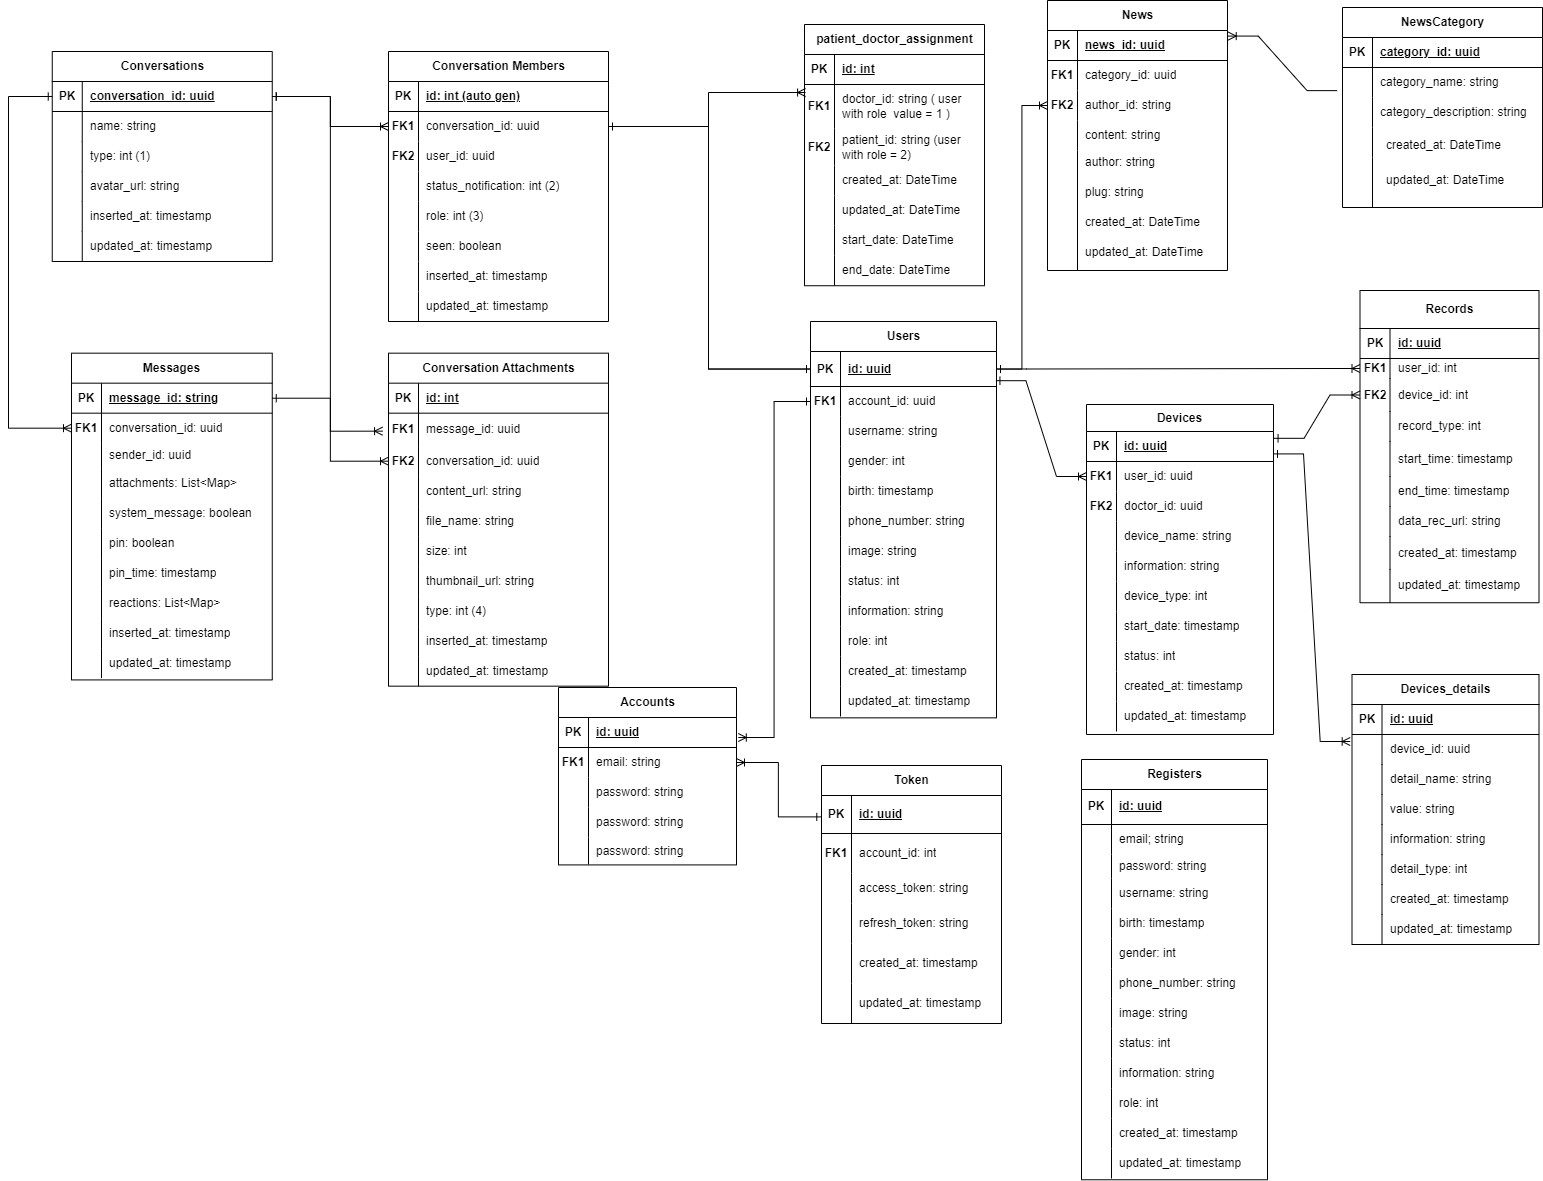
\includegraphics[width=15cm,height=15cm]{Images/system/fmECG_database.png}
	\caption[Sơ đồ ERD]{\bfseries \fontsize{12pt}{0pt}\selectfont Sơ đồ ERD}
	\label{fmECG_architecture-Database}
\end{figure}

\subsection{Thiết kế giao diện}

\subsection{Thiết kế các chức năng cho website và server}

\subsubsection{Thiết kế API}


% \begin{enumerate}[a)]
%   \item API xác thực người dùng

%   \begin{xltabular}{\textwidth}{
%     | >{\raggedright\arraybackslash}p{4.5cm}
%     | >{\centering\arraybackslash}m{2.8cm}
%     | >{\raggedright\arraybackslash}X |
%     }
%     \caption{\bfseries \fontsize{12pt}{0pt}\selectfont Bảng API xác thực người dùng}
%     \label{table_api_auth}
%     \\
%     \hline
%     \bfseries Đường dẫn    &\bfseries Phương thức    &\bfseries Mô tả\\ \hline
%     api/auth/register   &   POST  & Đăng ký tài khoản \\ \hline
%   api/auth/login   &    POST    & Đăng nhập vào hệ thống \\ \hline
%   api/auth/logout   &    POST    & Đăng xuất khỏi hệ thống \\ \hline
%   api/auth/reset-password  &     POST   &  Gửi reset link kèm reset token đến email của người dùng để thay đổi mật khẩu \\  \hline
%   api/auth/reset-password/reset &   POST     &  Thay đổi lại mật khẩu với mã token được nhận  \\ \hline
%   \end{xltabular}

%   \item API xét duyệt đăng ký tài khoản

%   \begin{xltabular}{\textwidth}{
%     | >{\raggedright\arraybackslash}p{4cm}
%     | >{\centering\arraybackslash}m{2.8cm}
%     | >{\raggedright\arraybackslash}X |
%     }
%     \caption{\bfseries \fontsize{12pt}{0pt}\selectfont Bảng API xét duyệt đăng ký tài khoản}
%     \label{table_api_register}
%     \\
%     \hline
%     \bfseries Đường dẫn    &\bfseries Phương thức    &\bfseries Mô tả\\ \hline
%     api/register/list   &   GET  & Lấy danh sách các tài khoản đang chờ phê duyệt \\ \hline
%     api/register/accepted   &    POST    & Phê duyệt tài khoản đăng ký \\ \hline
%     api/register/rejected  &     POST   &  Từ chối phê duyệt tài khoản đăng ký \\  \hline  
%   \end{xltabular}

%   \item API quản lý thông tin người dùng

%   \begin{xltabular}{\textwidth}{
%     | >{\raggedright\arraybackslash}p{4cm}
%     | >{\centering\arraybackslash}m{2.8cm}
%     | >{\raggedright\arraybackslash}X |
%     }
%     \caption{\bfseries \fontsize{12pt}{0pt}\selectfont Bảng API quản lý thông tin người dùng}
%     \label{table_api_user}
%     \\
%     \hline
%     \bfseries Đường dẫn    &\bfseries Phương thức    &\bfseries Mô tả\\ \hline
%     api/user   &   GET  &  Lấy danh sách thông tin của tất cả người dùng \\  \hline
%    api/user/id/:userId  &   GET     & Lấy thông tin cụ thể của người dùng theo Id \\ \hline
%    api/user/role/:role  &   GET     & Lấy danh sách người dùng theo chức vụ \\ \hline
%    api/user/update   &    POST    &  Cập nhật thông tin người dùng \\  \hline
%    api/user/delete/:userId  &   DELETE     & Xóa thông tin người dùng theo Id \\ \hline
%   \end{xltabular}

% \item API quản lý thiết bị
% \begin{xltabular}{\textwidth}{
%   | >{\raggedright\arraybackslash}p{4.8cm}
%   | >{\centering\arraybackslash}m{2.8cm}
%   | >{\raggedright\arraybackslash}X |
%   }
%   \caption{\bfseries \fontsize{12pt}{0pt}\selectfont Bảng API quản lý thiết bị}
%   \label{table_api_device}
%   \\
%   \hline
%   \bfseries Đường dẫn    &\bfseries Phương thức    &\bfseries Mô tả\\ \hline
%   api/device   &   GET  & Lấy danh sách thông tin tất cả thiết bị \\ \hline
%   api/devide/:deviceId   &    GET    & Lấy thông tin của một thiết bị \\ \hline
%   api/device/add &   POST     & Thêm thông tin thiết bị mới \\ \hline
%   api/device/update  &     POST   & Cập nhật thông tin một thiết bị \\ \hline
%   api/device/delete/:deviceId  &     DELETE   & Xóa thông tin một thiết bị theo Id \\ \hline
% \end{xltabular}

% \item API quản lý bản ghi ECG
% \begin{xltabular}{\textwidth}{
%   | >{\raggedright\arraybackslash}p{5cm}
%   | >{\centering\arraybackslash}m{2.8cm}
%   | >{\raggedright\arraybackslash}X |
%   }
%   \caption{\bfseries \fontsize{12pt}{0pt}\selectfont Bảng API quản lý bản ghi ECG}
%   \label{table_api_ecg}
%   \\
%   \hline
%   \bfseries Đường dẫn    &\bfseries Phương thức    &\bfseries Mô tả\\ \hline
%  api/record   &   GET  & Lấy danh sách thông tin các phiên đo ECG \\ \hline
%  api/record/user/:userId   &    GET    & Lấy danh sách thông tin các phiên đo ECG của bệnh nhân \\ \hline
%  api/record/doctor/:doctorId &   GET     & Lấy danh sách thông tin các phiên đo ECG của các bệnh nhân được quản lý bởi bác sĩ \\ \hline
%  api/record/id/:recordId  &     GET   & Lấy thông tin một phiên đo của bệnh nhân \\ \hline
%  api/record/getData/:recordId  &     GET   & Lấy dữ liệu một phiên đo của bệnh nhân \\ \hline
%  api/ record/download/:recordId  &     GET   & Tải dữ liệu một phiên đo của bệnh nhân \\ \hline
%  api/record/update  &     POST   & Cập nhật thông tin một phiên đo của bệnh nhân \\ \hline
%  api/record/delete/:recordId  &     DELETE   & Xóa thông tin một phiên đo của bệnh nhân \\ \hline
%   \end{xltabular}


% \item API quản lý phân công bệnh sĩ - bệnh nhân
% \begin{xltabular}{\textwidth}{
%   | >{\raggedright\arraybackslash}p{4.5cm}
%   | >{\centering\arraybackslash}m{2.8cm}
%   | >{\raggedright\arraybackslash}X |
%   }
%   \caption{\bfseries \fontsize{12pt}{0pt}\selectfont Bảng API quản lý phân công bác sĩ - bệnh nhân}
%   \label{table_api_pda}
%   \\
%   \hline
%   \bfseries Đường dẫn    &\bfseries Phương thức    &\bfseries Mô tả\\ \hline
%   api/pda   &   GET  & Lấy danh sách tất cả thông tin phân công bác sĩ - bệnh nhân \\ \hline
%   api/pda/create  &    POST    & Tạo một phân công bác sĩ - bệnh nhân mới \\ \hline
%   api/pda/update  &    POST    & Cập nhật thông tin một phân công bác sĩ - bệnh nhân mới \\ \hline
%   api/pda/delete/:pdaId  &    DELETE    & Xóa một phân công bác sĩ - bệnh nhân mới \\ \hline
%   api/pda/patient/:doctorId &  GET  & Lấy danh sách tất cả bệnh nhân theo ID bác sĩ \\ \hline
%   api/pda/doctor/:patientId &  GET  & Lấy danh sách tất cả bác sĩ theo ID bệnh nhân \\ \hline
%   \end{xltabular}

% \end{enumerate}




\subsubsection{Sơ đồ tuần tự API}

% ------------------------Auth----------------------



\subsection{Kết luận chương}

Chương 3 trình bày chi tiết về quá trình thiết kế hệ thống, bao gồm kiến trúc tổng thể và các thành phần cụ thể.
Thiết kế hệ thống tập trung vào việc xây dựng kiến trúc vận hành hiệu quả và mượt mà, chú trọng vào tính bảo mật, hiệu suất và khả năng mở rộng tối ưu.
\newpage